
% -- --------------------------------------------------------------------------------------------------- -- %
% -- Proyecto:                                                                                           -- %
% -- Archivo: reporte.rnw                                                                                -- %
% -- Repositorio: https://github.com/IFFranciscoME/A1_Temporal_Patterns                                  -- %
% -- Autor: Francisco ME                                                                                 -- %
% -- --------------------------------------------------------------------------------------------------- -- %

\documentclass{iteraposter}\usepackage[]{graphicx}\usepackage[]{color}
% maxwidth is the original width if it is less than linewidth
% otherwise use linewidth (to make sure the graphics do not exceed the margin)
\makeatletter
\def\maxwidth{ %
  \ifdim\Gin@nat@width>\linewidth
    \linewidth
  \else
    \Gin@nat@width
  \fi
}
\makeatother

\definecolor{fgcolor}{rgb}{0.345, 0.345, 0.345}
\newcommand{\hlnum}[1]{\textcolor[rgb]{0.686,0.059,0.569}{#1}}%
\newcommand{\hlstr}[1]{\textcolor[rgb]{0.192,0.494,0.8}{#1}}%
\newcommand{\hlcom}[1]{\textcolor[rgb]{0.678,0.584,0.686}{\textit{#1}}}%
\newcommand{\hlopt}[1]{\textcolor[rgb]{0,0,0}{#1}}%
\newcommand{\hlstd}[1]{\textcolor[rgb]{0.345,0.345,0.345}{#1}}%
\newcommand{\hlkwa}[1]{\textcolor[rgb]{0.161,0.373,0.58}{\textbf{#1}}}%
\newcommand{\hlkwb}[1]{\textcolor[rgb]{0.69,0.353,0.396}{#1}}%
\newcommand{\hlkwc}[1]{\textcolor[rgb]{0.333,0.667,0.333}{#1}}%
\newcommand{\hlkwd}[1]{\textcolor[rgb]{0.737,0.353,0.396}{\textbf{#1}}}%
\let\hlipl\hlkwb

\usepackage{framed}
\makeatletter
\newenvironment{kframe}{%
 \def\at@end@of@kframe{}%
 \ifinner\ifhmode%
  \def\at@end@of@kframe{\end{minipage}}%
  \begin{minipage}{\columnwidth}%
 \fi\fi%
 \def\FrameCommand##1{\hskip\@totalleftmargin \hskip-\fboxsep
 \colorbox{shadecolor}{##1}\hskip-\fboxsep
     % There is no \\@totalrightmargin, so:
     \hskip-\linewidth \hskip-\@totalleftmargin \hskip\columnwidth}%
 \MakeFramed {\advance\hsize-\width
   \@totalleftmargin\z@ \linewidth\hsize
   \@setminipage}}%
 {\par\unskip\endMakeFramed%
 \at@end@of@kframe}
\makeatother

\definecolor{shadecolor}{rgb}{.97, .97, .97}
\definecolor{messagecolor}{rgb}{0, 0, 0}
\definecolor{warningcolor}{rgb}{1, 0, 1}
\definecolor{errorcolor}{rgb}{1, 0, 0}
\newenvironment{knitrout}{}{} % an empty environment to be redefined in TeX

\usepackage{alltt}

\usepackage{lipsum}                                % Dummy text
\usepackage[absolute, overlay]{textpos}            % Figure placement
\setlength{\TPHorizModule}{\paperwidth}
\setlength{\TPVertModule}{\paperheight}


\title{
  Clustering subsecuencial de series de tiempo: Evidencia de patrones temporales en el
  tipo de cambio USD/MXN
  }

\vskip4cm

\author {
  Msc. Juan Francisco Mu\~noz Elguez\'abal \inst{1}
  \and
  Dr. Riemann Ru\'iz Cruz \inst{2}
  }

\institute {
  \inst{1} Msc. Ciencia de Datos - ITESO
  \and
  \inst{2} Departamento de Matem\'aticas y F\'isca - ITESO
  }

% -- --------------------------------------------------------------------------- Comienzo de codigo en R -- %










\IfFileExists{upquote.sty}{\usepackage{upquote}}{}
\begin{document}

\begin{frame}

\begin{columns}[onlytextwidth]

  \begin{column}{.6\textwidth - 0.01\textwidth}
    \begin{block}{Descripci\'on General}
      Metodolg\'ia \textit{BoxJenkins} para series de tiempo financieras. Modelo lineal 
      univariado que utiliza informaci\'on end\'ogena de la serie de tiempo para construir un modelo 
      matem\'atico con el cual realizar predicciones de valores futuros.
    \end{block}
    
    \begin{block}{Diagrama General}
      \begin{figure}[H]
        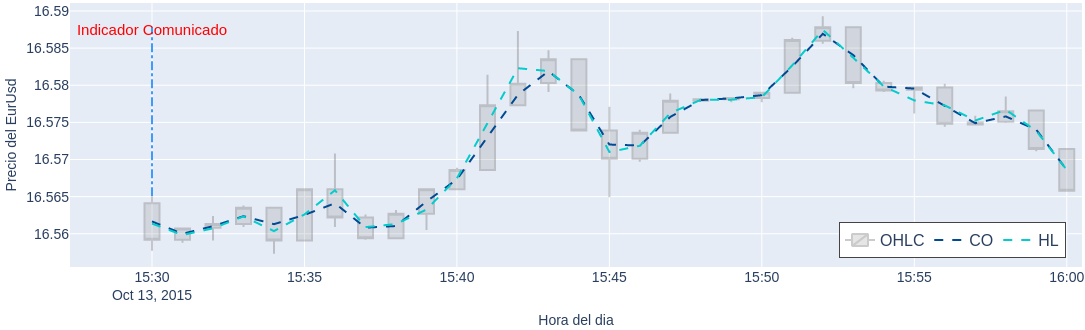
\includegraphics[scale=1]{imagenes/grafica_1.png}
      \end{figure}
    \end{block}
\end{column}

\begin{column}{.4 \textwidth - 0.01\textwidth}
  \begin{block}{Tabla General}
     
\begin{tabular}{c|c|c}
\hline
id & pais & ocurrencias\\
\hline
12-Monlation\_MEX & MEX & 104\\
\hline
1sthallation\_MEX & MEX & 105\\
\hline
3-Montuction\_USA & USA & 392\\
\hline
3-Yearuction\_USA & USA & 91\\
\hline
30-Yeauction\_USA & USA & 96\\
\hline
4-Weekuction\_USA & USA & 391\\
\hline
6-Montuction\_USA & USA & 395\\
\hline
ADPEmpChange\_USA & USA & 120\\
\hline
APIWeelStock\_USA & USA & 235\\
\hline
AccumuuntGDP\_MEX & MEX & 36\\
\hline
AveragngsMoM\_USA & USA & 120\\
\hline
AveragngsYoY\_USA & USA & 118\\
\hline
AveragyHours\_USA & USA & 120\\
\hline
BakerHgCount\_USA & USA & 235\\
\hline
BuildiChange\_USA & USA & 47\\
\hline
BuildiitsMoM\_USA & USA & 121\\
\hline
Businetories\_USA & USA & 120\\
\hline
CFTCGoitions\_USA & USA & 205\\
\hline
CFTCOiitions\_USA & USA & 205\\
\hline
CFTCUSitions\_USA & USA & 206\\
\hline
Capacization\_USA & USA & 120\\
\hline
CentrastRate\_MEX & MEX & 67\\
\hline
ChalleobCuts\_USA & USA & 96\\
\hline
ChicagyIndex\_USA & USA & 120\\
\hline
Chicag'Index\_USA & USA & 100\\
\hline
ConstringMoM\_USA & USA & 120\\
\hline
Consumidence\_MEX & MEX & 120\\
\hline
Consumnces.a\_MEX & MEX & 120\\
\hline
ConsumChange\_USA & USA & 120\\
\hline
Consumores.a\_USA & USA & 103\\
\hline
ConsumdexMoM\_USA & USA & 104\\
\hline
ConsumdexYoY\_USA & USA & 96\\
\hline
ConsumrgyMoM\_USA & USA & 120\\
\hline
ConsumrgyYoY\_USA & USA & 120\\
\hline
Consums.aMoM\_USA & USA & 96\\
\hline
ContinClaims\_USA & USA & 521\\
\hline
CoreInlation\_MEX & MEX & 102\\
\hline
CorePediture\_USA & USA & 239\\
\hline
CorePeresQoQ\_USA & USA & 116\\
\hline
Currenccount\_USA & USA & 40\\
\hline
Currennt,QoQ\_MEX & MEX & 36\\
\hline
DallassIndex\_USA & USA & 95\\
\hline
DurablOrders\_USA & USA & 122\\
\hline
Durablefense\_USA & USA & 15\\
\hline
Durabltation\_USA & USA & 122\\
\hline
EIACruChange\_USA & USA & 521\\
\hline
EIANatChange\_USA & USA & 408\\
\hline
EmploytIndex\_USA & USA & 35\\
\hline
ExistingeMoM\_USA & USA & 120\\
\hline
ExistilesMoM\_USA & USA & 119\\
\hline
ExportdexMoM\_USA & USA & 105\\
\hline
ExportdexYoY\_USA & USA & 94\\
\hline
FactorersMoM\_USA & USA & 120\\
\hline
FedIntcision\_USA & USA & 80\\
\hline
Fiscal,pesos\_MEX & MEX & 101\\
\hline
GoodsTalance\_USA & USA & 55\\
\hline
GrossDalized\_USA & USA & 119\\
\hline
GrossDeIndex\_USA & USA & 119\\
\hline
GrossDuctQoQ\_MEX & MEX & 37\\
\hline
GrossDuctYoY\_MEX & MEX & 37\\
\hline
Headlilation\_MEX & MEX & 103\\
\hline
HousinChange\_USA & USA & 48\\
\hline
HousinrtsMoM\_USA & USA & 120\\
\hline
IBDTIPismMoM\_USA & USA & 119\\
\hline
ISMManingPMI\_USA & USA & 93\\
\hline
ISMManesPaid\_USA & USA & 118\\
\hline
ISMNoningPMI\_USA & USA & 120\\
\hline
ISM-NYsIndex\_USA & USA & 120\\
\hline
ImportdexMoM\_USA & USA & 120\\
\hline
IndustputMoM\_MEX & MEX & 120\\
\hline
IndustputYoY\_MEX & MEX & 104\\
\hline
IndustionMoM\_USA & USA & 104\\
\hline
InitiaClaims\_USA & USA & 520\\
\hline
LaborFonRate\_USA & USA & 72\\
\hline
MarkitingPMI\_USA & USA & 145\\
\hline
Markitposite\_USA & USA & 184\\
\hline
MarkitcesPMI\_USA & USA & 134\\
\hline
MichigtIndex\_USA & USA & 240\\
\hline
Monthltement\_USA & USA & 120\\
\hline
NAHBHotIndex\_USA & USA & 120\\
\hline
NFIBBumIndex\_USA & USA & 95\\
\hline
NYEmpigIndex\_USA & USA & 120\\
\hline
NetLonCFlows\_USA & USA & 120\\
\hline
NewHomngeMoM\_USA & USA & 120\\
\hline
NewHomlesMoM\_USA & USA & 120\\
\hline
Nonfaryrolls\_USA & USA & 79\\
\hline
Nonfartivity\_USA & USA & 120\\
\hline
PendinlesYoY\_USA & USA & 88\\
\hline
Personitures\_USA & USA & 88\\
\hline
PersoncesQoQ\_USA & USA & 95\\
\hline
PersonomeMoM\_USA & USA & 237\\
\hline
Personending\_USA & USA & 120\\
\hline
PhiladSurvey\_USA & USA & 120\\
\hline
PrivatingQoQ\_MEX & MEX & 30\\
\hline
PrivatingYoY\_MEX & MEX & 30\\
\hline
ProducdexMoM\_USA & USA & 120\\
\hline
ProducdexYoY\_USA & USA & 120\\
\hline
ProducrgyMoM\_USA & USA & 119\\
\hline
ProducrgyYoY\_USA & USA & 119\\
\hline
RedboodexMoM\_USA & USA & 390\\
\hline
RedboodexYoY\_USA & USA & 390\\
\hline
RetaillGroup\_USA & USA & 60\\
\hline
RetaillesMoM\_MEX & MEX & 104\\
\hline
RetaillesMoM\_USA & USA & 120\\
\hline
RetaillesYoY\_MEX & MEX & 104\\
\hline
RetailtosMoM\_USA & USA & 120\\
\hline
SPCasecesYoY\_USA & USA & 120\\
\hline
TotalNCFlows\_USA & USA & 120\\
\hline
TradeBalance\_USA & USA & 119\\
\hline
TradeBncesa,\_MEX & MEX & 105\\
\hline
TradeBlance,\_MEX & MEX & 106\\
\hline
UnemplntRate\_USA & USA & 120\\
\hline
UnitLarCosts\_USA & USA & 79\\
\hline
Wholestories\_USA & USA & 154\\
\hline
\end{tabular}


  \end{block}
\end{column}
  
\end{columns}



\end{frame}
\end{document}
